../preamble/preamble.tex
\usepackage{pdfpages}
%\usepackage{spconf}

%\addbibresource{main.bib}

\newcommand\fullsum{\sum\limits_{n=1}^{N} \sum\limits_{m=1}^{M}}
\newcommand\fullphase{\omega_{nm}t + \vec \kappa_{nm}\vec r_0 + \psi_{nm}}
% Title.
% ------
%\title{}
%
% Single address.
% ---------------
%\name{Author(s) Name(s)\thanks{Thanks to XYZ agency for funding.}}
%\address{Author Affiliation(s)}
%
% For example:
% ------------
%\address{School\\
%	Department\\
%	Address}
%
% Two addresses (uncomment and modify for two-address case).
% ----------------------------------------------------------
%\twoauthors
%  {A. Author-one, B. Author-two\sthanks{Thanks to XYZ agency for funding.}}
%	{School A-B\\
%	Department A-B\\
%	Address A-B}
%  {C. Author-three, D. Author-four\sthanks{The fourth author performed the work
%	while at ...}}
%	{School C-D\\
%	Department C-D\\
%	Address C-D}

%\title{Черновик статьи \\ \textbf{Моделирование измерения
%ЭПР инструментом DPR/GMI на модели заостренной морской
%поверхности}}
%\author{Понур К.А.}
\begin{document}

\begin{titlepage}
    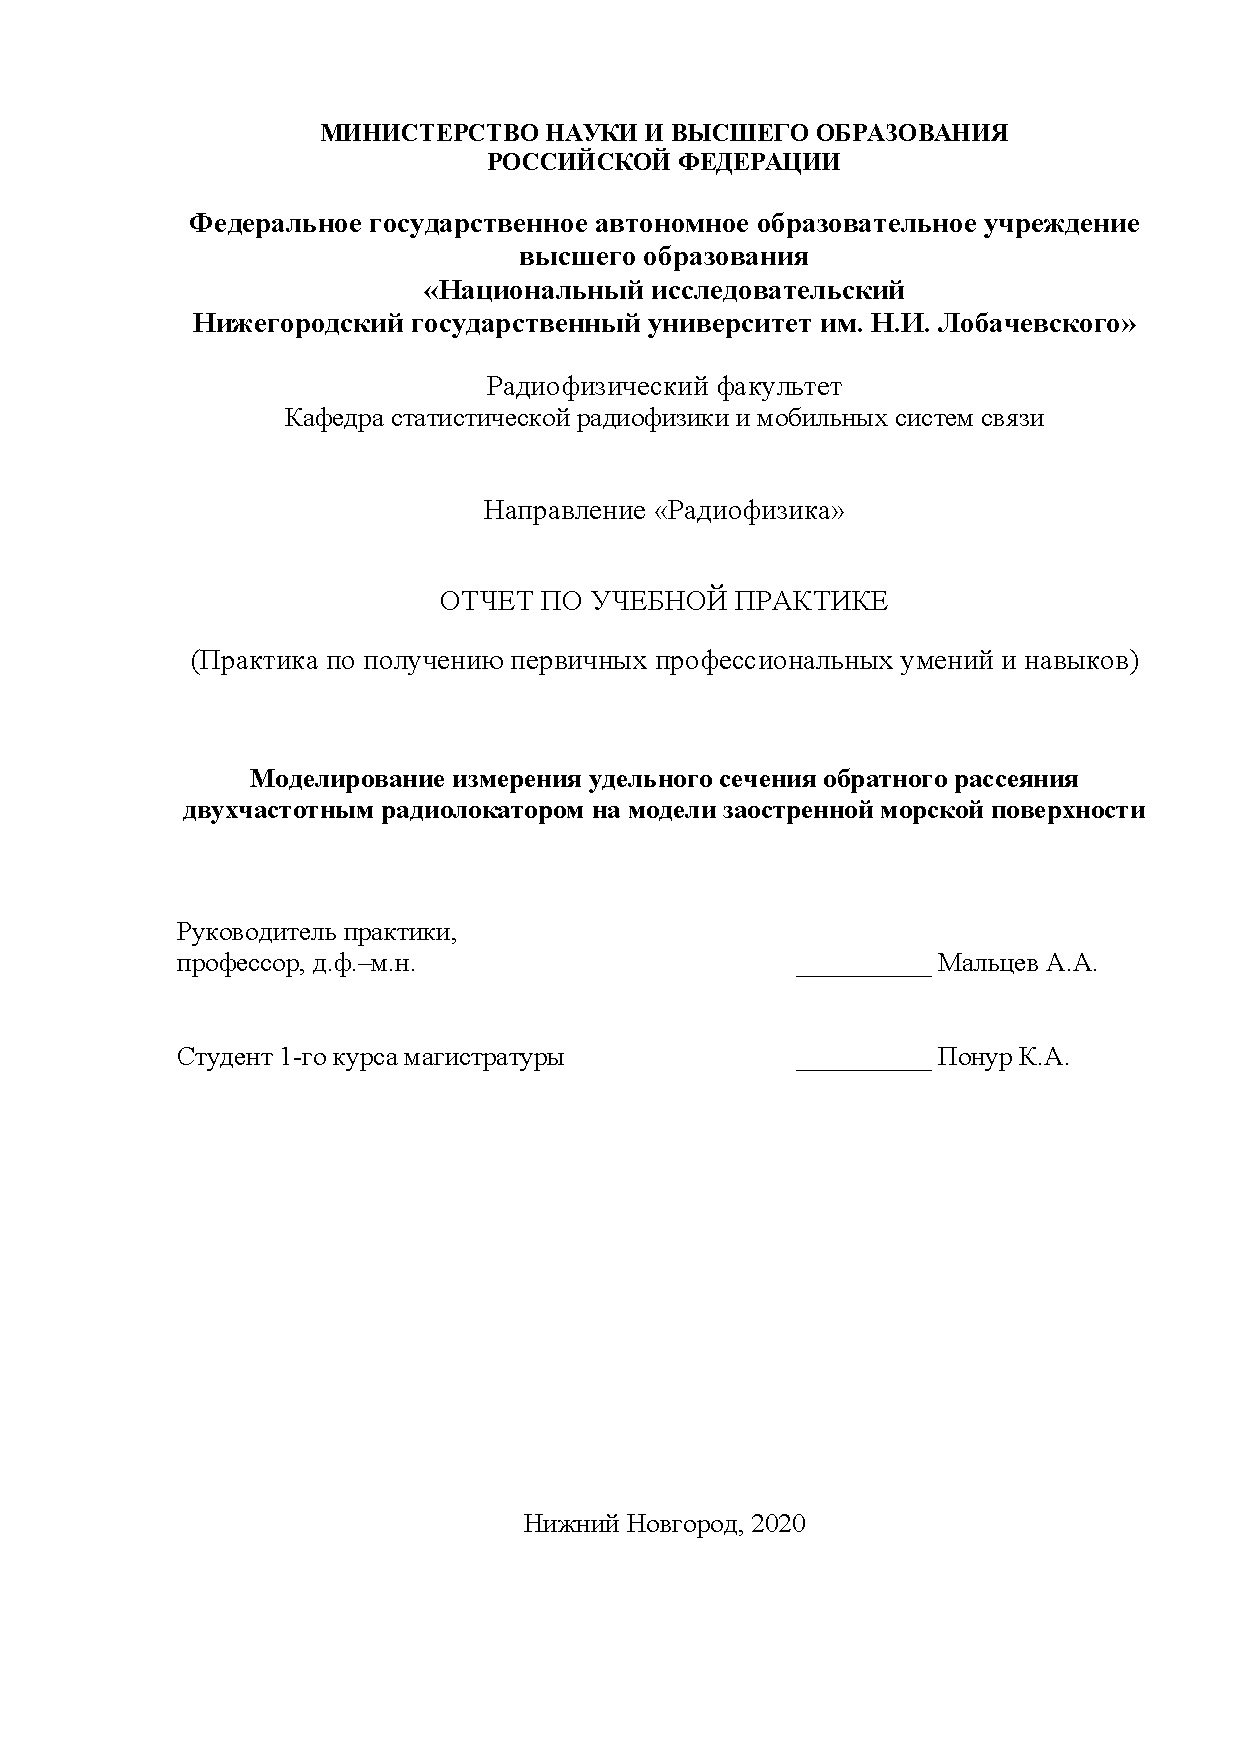
\includepdf{title_report2021.pdf}
\end{titlepage}
%\begin{abstract}
%The abstract should appear at the top of the left-hand column of text, about
%0.5 inch (12 mm) below the title area and no more than 3.125 inches (80 mm) in
%length.  Leave a 0.5 inch (12 mm) space between the end of the abstract and the
%beginning of the main text.  The abstract should contain about 100 to 150
%words, and should be identical to the abstract text submitted electronically
%along with the paper cover sheet.  All manuscripts must be in English, printed
%in black ink.
%\end{abstract}
%
%\begin{keywords}
%One, two, three, four, five
%\end{keywords}

%\maketitle



%\maketitle
%\newpage
\section*{Введение}
Моделирование морской поверхности является важной и активно развивающимся
направлением, но несмотря на это остается ряд вопросов, которые требуют дальнейших исследований в приложении к решаемой
задаче. 

В настоящее время активно применяются модели третьего поколения, наиболее
известные из которых модели WAM (WaveModel), SWAN (Simulation Waves Nearshore)
и WaveWatch III \cite{wavewatch3, swan, wam4}.  Для описания поверхностного
волнения эти модели применяют уравнения гидродинамики, но в общем виде задача
пока не по силам современной вычислительной технике. Благодаря упрощениям и
предположениям задача становится «счетной», но требует слишком много
вычислительных ресурсов, поэтому этот подход используется для решения
научно-исследовательских задач, например, \cite{slunyaev2006, slunyaev2009,
west1987}. 

В данной работе на модельной морской поверхности будет решаться задача
обратного рассеяния электромагнитного излучения.  При её решении необходимо
найти отраженное поля вблизи приемной антенны, а для этого необходимо выполнить
интегрирование по всей рассеивающей площадке.  Для получения точного результата в результате интегрирования необходимо
обеспечить шаг по поверхности в несколько раз меньше длины волны излучения
\cite{toporkov:brown:2000, toporkov:brown:2002}. Для типичного пятна GMI необходимо будет построить
модель поверхности
размером 25 км$^2$ с разрешением порядка $0.2$ см, вычисление на такой
поверхности двумерного интеграла занимает слишком много времени на современной
технике. К тому же само моделирование поверхности такого размера является
сложной задачей для моделей, опирающихся на уравнения гидродинамики. 

Для оценки эффективности работы радиолокационной аппаратуры
больше подходит хорошо известный подход, опирающийся на модель спектра
волнения, например, \cite{longe-higgins}. В этом случае морская поверхность представляется в
виде набора гармоник, амплитуда которых вычисляется по спектру волнения. При
таком подходе смоделированная морская поверхность утрачивает ряд свойств,
присущих реальной морской поверхности, но становится более удобной для счета и
моделирование может быть проведено на современном настольном компьютере за
приемлемое время. Именно этот подход выбран для моделирования морской поверхности в данной работе. 

Однако смоделированная одними лишь гармоническими функциями будет симметрична
и иметь нулевое среднее. Из экспериментов \cite{shuleykin} известно, что
настоящая морская поверхность имеет более острые вершины и пологие впадины, по
сравнению с синусоидами. Поэтому в данной работе используется модель
заостренной поверхности (CWM) \cite{nouguier}.


Надо отметить, что для выбранного подхода
качество моделирования зависит от используемого спектра волнения и от численной
реализации процедуры моделирования. Был выбран спектр \cite{ryabkova},
учитывающий короткие волны, играющие особую роль в задачах рассеяния.


\section*{Моделирование волнения}%

Обычный способ моделирования морской поверхности по известному спектру волнения
заключается в суммировании гармоник с детерменированными амплитудами и
случайными фазами. Поле возвышений в этом случае \where*{$\zeta$}{поле
возвышений} представляется в виде
\begin{equation}
    \label{eq:surface3d_default}
    \zeta(\vec r_0,t) = \fullsum A_n(\vec \kappa_{nm}) \cos(\fullphase),    \\
\end{equation}
где \where{$\vec \kappa$}{двумерный волновой вектор},  
$\vec r_0 = (x_0, y_0)$, $\vec r = (x, y)$, 
\where{$\psi_{nm}$}{случайная фаза равномерно распределенная в интервале от $0$ до $2 \pi$}, 

\where{$A_n (\vec \kappa_n)$}{амплитуда гармоники с волновым
вектором}, вычисляемая по известному спектру волнения \cite{ryabkova},
$\vec \kappa_n$ и временной частотой
\where*{$\omega_n(\kappa_{nm})$}{дисперсионное соотношение} \cite{pustovoytenko}.


Известно что в глубоком море
поверхностные частицы на волнах описывают окружность (см. \cite{shuleykin}).
Следовательно саму волну правильнее описывать параметрическим уравнением
трохоиды (см. \cite{nouguier})

\begin{equation}
    \begin{gathered}
        \label{eq:surface3d_cwm}
        x(\vec r,t) = x_0 - \fullsum A_n(\vec \kappa_{nm})\frac{\vec \kappa_x}{\kappa}        \sin(\fullphase)\\
        y(\vec r,t) = y_0 - \fullsum A_n(\vec \kappa_{nm}) \frac{\vec \kappa_y}{\kappa}
        \sin(\fullphase)\\
        \zeta(\vec r,t) = \fullsum
        A_n(\vec \kappa_{nm}) \cdot \cos(\fullphase)    \\
    \end{gathered}
\end{equation}

Наклоны поверхности в каждой точке можно найти дифференцируя
\eqref{eq:surface3d_cwm} 
\begin{equation}
    \begin{gathered}
        \xi_{x}(\vec r,t) = \pdv{\zeta(\vec r,t)}{x_0} = \fullsum \kappa_{x} A_n(\vec \kappa_{nm}) \cdot \sin(\fullphase)    \\
        \xi_{y}(\vec r,t) = \pdv{\zeta(\vec r,t)}{y_0} = \fullsum  \kappa_{y} A_n(\vec \kappa_{nm}) \cdot \sin(\fullphase)    \\
    \end{gathered}
\end{equation}

%На рис. \ref{fig:cwm_demo} показано как преобразуется одна гармоническая
%функция в результате преобразования в модель заостренной поверхности. Эффект
%заострения на рис. \ref{fig:cwm_demo} усилен для наглядности. 

Сравнение заостренной морской поверхности с обычной представлено на рис.
\ref{fig:cwm_modeling}. Из рис. \ref{fig:cwm_modeling} заметно, что модель
заостренной поверхности оказывает большое влияние на наклоны поверхности, что
скажется на решения задач рассеяния.


%\begin{figure}[H]
%\centering
%\makeatletter
    %\@for\i:={1,2}\do{
    %\begin{subfigure}{0.45\textwidth}
        %\centering
        %\includegraphics[width=\linewidth, page=\i]{figs/cwm_demo}
        %\subcaption{}
        %\label{subfig:cwm_demo\i}
    %\end{subfigure}
%}


%\caption{
    %Сравнение характеристик заостренной и обычной поверхностей на примере одной
    %синусоиды (эффект заострения усилен для наглядности): \\
    %\subref{subfig:cwm_demo1} поле высот;
    %\subref{subfig:cwm_demo2} поле полных наклонов;
    %Синей линией отмечена синусоида, оранжевой -- трохоида.
%}
%\makeatother
%\label{fig:cwm_demo}
%\end{figure}



\begin{figure}[H]
\centering
\makeatletter
    \@for\i:={1,2,3}\do{
    \begin{subfigure}{0.45\textwidth}
        \centering
        \includegraphics[width=\linewidth, page=\i]{figs/cwm_demo_1d}
        \subcaption{}
        \label{subfig:cwm_modeling\i}
    \end{subfigure}
    %\hfill
}


\caption{
    Сравнение основных характеристик реализаций заостренной и обычной
    морских поверхностей: \\
    \subref{subfig:cwm_modeling1} поле высот;
    \subref{subfig:cwm_modeling2} поле наклонов вдоль направления
    распространения волнения;
    \subref{subfig:cwm_modeling3} поле наклонов перпендикулярное направлению
    распространения волнения;
    Синей линией отмечена обычная поверхность, оранжевой -- заостренная.
}

\makeatother
\label{fig:cwm_modeling}
\end{figure}



\subsection*{GPM}%
\label{sub:GPM}

На предложенной выше модели волнения будет проводиться эксперимент с японским
спутником Global Precipitation Measurement (GPM). Проект GPM
 является продолжением и расширением
спутника наблюдения за тропическими осадками (TRMM) и
международной миссии по подробному измерению глобальных осадков для
уточнения изменений климата и течений с использованием одного основного
спутника GPM с двухчастотным радиолокатором осадков (DPR) и микроволнового
радиометра (GMI) на борту и нескольких других спутников с микроволновым
радиометром на борту.

%The Global Precipitation Measurement Project (GPM) is follow-on and expansion
%of the tropical rain observation satellite (TRMM) satellite, and an
%international cooperative mission to measure global precipitation more
%accurately and frequently for elucidating changes in climate and water
%circulation using one GPM core satellite with the Dual-frequency
%Precipitation Radar (DPR) and the GPM Microwave Imager (GMI) onboard and
%constellation of several other satellites with a microwave imager onboard. 

\begin{table}[H]
    \centering
    \begin{tabular}{|c|c|}
        \hline
        Характеристика & Значение\\
        \hline
        Время запуска & 27 февраля 2014 \\
        Высота & $\approx 407$ км\\
        Наклон оси & $\approx 64^{\circ}$ \\
        Радиус главной полуоси & $\approx 6776 \text{ км}$ \\
        Инструменты & DPR, GPM \\
        Масса & $\approx 3850$ кг \\
        Габариты &  $13.0 \text{ м} \times 6.5 \text{ м} \times 5.0 \text{
        м}$\\
        \hline
    \end{tabular}
    \caption{Технические характеристики GPM}
    \label{tab:GPM}
\end{table}

\begin{figure}[h]
    \centering
    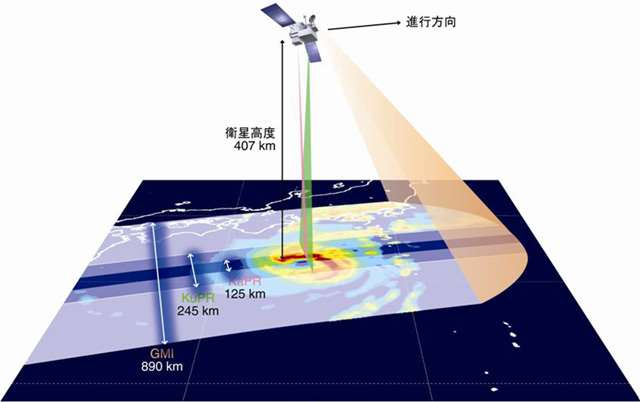
\includegraphics[width=0.6\linewidth]{figs/gpm.png}
    \caption{Схема измерения GPM}
    \label{fig:GPM}
\end{figure}

%Прибор измеряет под малыми углами падения от -17 до 17 градусов, что является
%необыч

%Цель

\subsubsection*{Вычисление УЭПР}%

%В данной работе будет проводиться айти УЭПР в зависимости от углов падения.
Чтобы найти $\sigma$ ЭПР морской поверхности её для начала придется вычислить по
определению ЭПР 
\begin{equation}
    \sigma = 4 \pi R^2 \abs{\frac{E_2^2}{E_1^2}}
\end{equation}

Поле отраженной от поверхности сферической волны можно вычислить,
интегрируя по всей отражающей площадке $S$
\begin{equation}
    E_2 = \frac{1}{\lambda} \int\limits_{S} \frac{E_1}{R} G(\theta, \phi) \exp(-j \cdot 2 k R)
    \cos \theta \dd S,
\end{equation}
где $R$ -- расстояние от антенны до точки на площадке. 

%\begin{equation}
    %\frac{E_2}{E_1} = \frac{1}{\lambda} \exp(-j \cdot 2k R_0)
    %\int\limits_{S} \frac{1}{R} \exp{-j \cdot 2 k r } \dd S
%\end{equation}

\begin{equation}
    \label{eq:sigma}
    \sigma = \frac{4 \pi R^2}{\lambda^2} \abs{\int\limits_{S}^{} \frac{G(\theta,
            \phi)}{R} \exp{-j \cdot 2 k
    r } \cos \theta \dd S}^2
\end{equation}

Мы же будем работать с УЭПР, определяемой следующим образом
\begin{equation}
    \label{eq:crosssec}
    \sigma_0 =   \sigma \cdot \qty(\int\limits_S G(\theta, \phi) \dd S)^{-1},
\end{equation}
где $G(\theta, \phi)$ -- диаграмма направленности антенны.

Искать УЭПР для всей поверхности слишком сложно и ресурсоемко, поскольку
её точное вычисление требует счета двумерного интеграла по всей
рассеивающей площадке. Однако при малых углах падения, при которых
работает GPM, основной вклад вносит механизм зеркального отражения, поэтому мы
будем считать УЭПР только от точек, дающих максимальный вклад в отраженный
сигнал -- тех, для которых максимально скалярное произведение вектор $\vec R$ и
нормали к поверхности в текущей точке  $\vec n$: для зеркальных точек. Искать
все зеркальные точки мы тоже не в состоянии, поэтому будем искать только точки
из достаточно большой выборки. Если выборка получится достаточно большой, то
разницы между практикой не будет. 

При вышеуказанных предположениях, интеграл \eqref{eq:crosssec} разобьется на
сумму по выборке зеркальных точек, который для случая гауссовой морской
поверхности будет совпадать с известной теоретической формулой
\begin{equation}
    \label{eq:sigma0_theory}
    \sigma_0 = \frac{\abs{F(0)}^2}{\cos^4\theta \sqrt{\sigma_{xx}^2
    \sigma_{yy}^2 - K_{xy}^2(0)}} \exp{- \frac{\sigma^2_{xx}
    \tan^2\theta}{\sigma_{xx}^2 \sigma_{yy}^2 - K_{xy}^2(0)}}
\end{equation}

Спутник DPR работает в двух диапазонах, имеющих различные дисперсии наклонов.
Поскольку Ka-диапазон имеет волну, короче, чем Ku-диапазон, то в нём мы сможем
увидеть больше неровностей морской поверхности и меньшее количество зеркальных
площадок. Поэтому в Ka-диапазоне УЭПР при нулевом угле падения будет меньше,
чем в Ku-диапазоне.  Этот эффект предсказывает и теоретическая формула
\eqref{eq:sigma0_theory}. 
Распределение зеркальных точек в двух диапазонах для антенны, направленной
вертикально вниз представлено на рис. \ref{fig:mirror_dots_distrib}. 
Зеркальные точки при нулевом угле падения должны располагаться преимущественно
на пиках и впадинах поверхности, практически отсутствуя на склонах. Это также
отражает рис. \ref{fig:mirror_dots_distrib}.

Для выборки зеркальных точек  интеграл \eqref{eq:sigma} разбивается на сумму
площадей отдельных зеркальных площадок. 


%\begin{figure}[h]
    %\centering
    %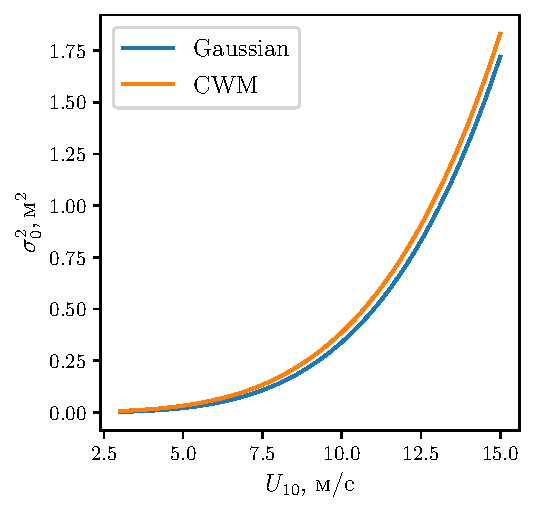
\includegraphics[width=0.6\linewidth]{figs/cwm_variance}
    %\caption{}
    %\label{fig:}
%\end{figure}




\begin{figure}[h]
    \centering
    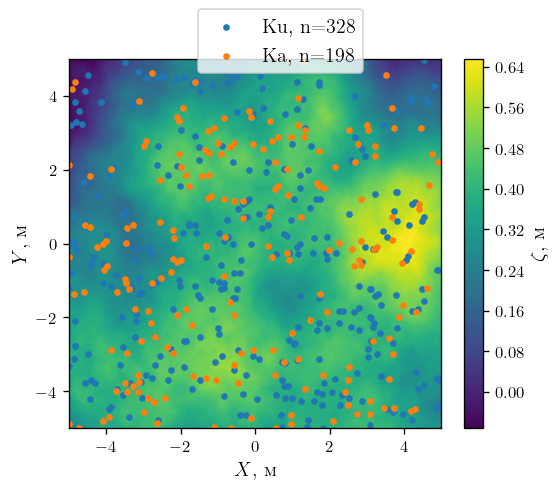
\includegraphics[width=0.6\linewidth]{figs/mirrordots.png}
    \caption{Распределение зеркальных точек на двумерной поверхности высот для
    Ku- и Ka-диапазонов, $n$--количество соответствующих точек на поверхности }
    \label{fig:mirror_dots_distrib}
\end{figure}

%\begin{figure}[h]
    %\centering
    %\includegraphics[width=0.6\linewidth]{figs/mirror_dots_Ku.png}
    %\caption{Распределение углов отклонения от направления
        %зеркального отражения для $Ku$-диапазона }
    %\label{fig:mirror_angles_distrib}
%\end{figure}

\subsection*{Численный эксперимент}%
\label{sub:chislennyi_eksperiment}


%\footnote{При углах > 12 в УЭПР нужно учитывать не только зеркалку, но и
%рассеяние и по-честному считать интеграл. Так ли это?}, 


Для валидации модели был взят один трек спутника (см. рис. \ref{fig:track_dpr} ) и произведено сравнение срезов трека с
модельными данными (см. рис. \ref{fig:crosssec}). 
Используемый метод моделирования и предположения, лежащие в его
основе не позволяют производить моделирование при углах отклонения антенны более чем $12^\circ$. 

Из рис. \ref{fig:crosssec} заметно, что УЭПР, полученная со спутника при росте
угла падения начинает различаться с теоретической \eqref{eq:crosssec}. 
Однако при моделировании заостренной поверхности мы можем точнее приблизить
модельную кривую к реальной

%\footnote{Усреднить модельные кривые за 100 срезов,
%чтобы выглядело красивее}
\begin{figure}
    \centering
    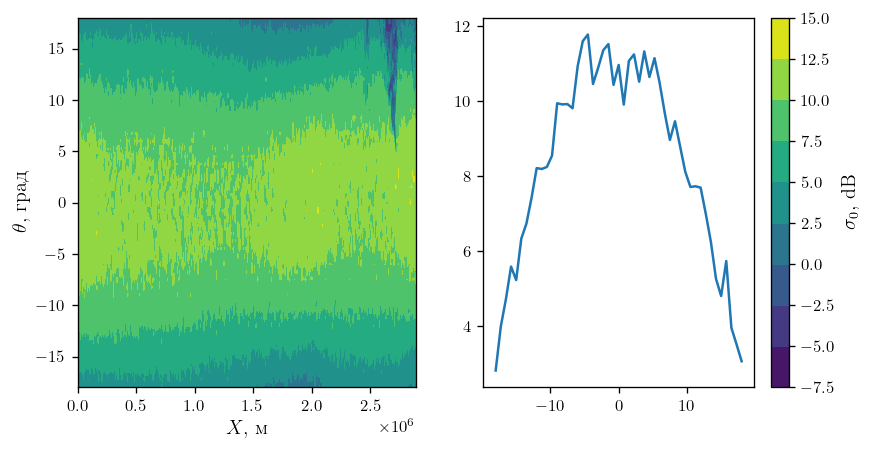
\includegraphics[width=0.8\linewidth]{figs/real_crosssec.png}
    \caption{Трек, полученный с DPR}
    \label{fig:track_dpr}
\end{figure}





%\newpage

%%\bibliography{main}
\newpage
\section*{Заключение}

\begin{figure}
    \centering
    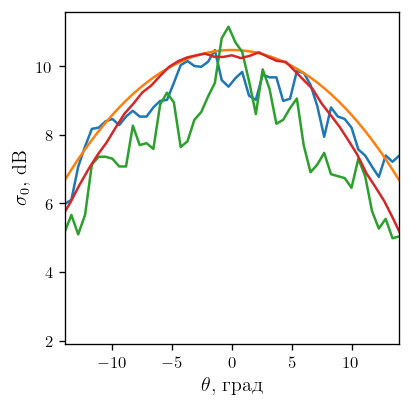
\includegraphics[width=0.6\linewidth]{figs/crosssec.png}
    \caption{Зависимость УЭПР $\sigma_0$ от угла падения  $\theta$; 
    оранжевой линией обозначено теоретическое значение УЭПР,
    синей -- УЭПР, посчитанная по одному срезу обычной морской поверхности,
    зеленой -- УЭПР, посчитанная по одному срезу заостренной морской поверхности,
    красной -- УЭПР, усредненная по 500 срезам DPR}
    \label{fig:crosssec}
\end{figure}

В данной работе на модельной морской поверхности решалась задача
обратного рассеяния электромагнитного излучения.  Для её решения 
искалось отраженное от зеркальных точек поле вблизи приемной антенны, а затем
моделировалось удельное сечение обратного рассеяния. Построенная модель хорошо
согласуется со спутниковыми и теоретическими данными.

\bibliographystyle{abbrv}
\bibliography{main}
%%\printnomenclature[5em]
\end{document}

